%\documentclass[urop]{socreport}
\documentclass[a4paper,11pt]{article}
%\usepackage{fullpage}
%\usepackage{fancyheadings}
\usepackage{tabularx}
\usepackage{graphics,lscape}
\usepackage{graphicx}
\usepackage{url}
\usepackage{verbatim}

\usepackage{lastpage}

%\usepackage{rotating}

%\pagestyle{headings}

\usepackage{fancyhdr}
\pagestyle{fancy}

\newenvironment{mylisting}
{\begin{list}{}{\setlength{\leftmargin}{1em}}\item\small\bfseries}
{\end{list}}

\vfuzz2pt % Don't report over-full v-boxes if over-edge is small
\hfuzz2pt % Don't report over-full h-boxes if over-edge is small

\lhead{Workpackage 1, Deliverable 1.1} %{text for header left} % no text within brackets gives empty space
\chead{} %{text for header centre}
\rhead{} %{text for header right} % text preceded by "/bfseries" would give bold text
\lfoot{\today} %{text for footer left}
\cfoot{} %{text for footer centre}
\rfoot{Page \thepage/\pageref{LastPage}} %{text for footer right} % the text "/thepage" would give page number
%\rfoot{}
\renewcommand{\headrulewidth}{0pt}
\renewcommand{\footrulewidth}{0pt}


%\setlength{\oddsidemargin}{0cm}
%\setlength{\evensidemargin}{0cm}
%\setlength{\textwidth}{16cm}
\setlength{\textheight}{23cm}


\begin{document}

% FRONT PAGE TO GO HERE

%\pagenumbering{roman}
%\title{Deliverable reference number and Title\\
%D1.1: X-Agent framework and software environment for agent-based
%models in economics}
%\author{Simon Coakley\\Mariam Kiran}
%\projyear{2006/07} \projnumber{035086} \advisor{Prof. Mike Holcombe}
%\deliverables{
%    \item Start Date: September 1st 2006
%    \item Duration: 36 months
%    \item Organisation name of lead contractor for this deliverable:
%University of Sheffield (\textbf{USFD})\\
%\begin{tabular}
%{|p{0.3in}|p{3.7in}|p{0.6in}|} \hline \multicolumn{3}{|p{5in}|}
%{\textbf{Project co-funded by the European
%Commission within the Sixth Framework Programme (2002-2006) }} \\
%\hline \multicolumn{3}{|p{3in}|}{\textbf{Dissemination Level }} \\
%\hline \textbf{PU } & Public  &  \\ \hline \textbf{PP } & Restricted
%to other programme participants (including the Commission Services)
%&  \\ \hline \textbf{RE } & Restricted to a group specified by the
%consortium (including the Commission Services)  &  \\ \hline
%\textbf{CO } & Confidential, only for members of the consortium
%(including the Commission Services)  &  \\ \hline
%\end{tabular}%}
%\maketitle

%\begin{abstract}

 %\vspace{2cm}

%This report presents the work completed for deliverable D1.1
%depicting how the X-agent framework FLAME facilitates use of agent
%based modelling in economics. This deliverable acts as part of the
%workpackage 1 which comprises of agent-based software engineering
%methodologies being laid down for the project EURACE.

%Keeping in accordance with milestone 1.1, the report presents a
%definition of the XMML modelling language and how it is used for
%economics and how agent-based models of economics can be written
%using it.


%\begin{descriptors}
 %   \item C5 Computer System Implementation
  %  \item G2.2 Graph Algorithms
%\end{descriptors}
%\begin{keywords}
 %   Problem, algorithm, implementation
%\end{keywords}
%\begin{implement}
 %   Solaris 10, g++ 3.3, Tcl/Tk 8.4.7
%\end{implement}
%\end{abstract}


%\begin{acknowledgement}
%\end{acknowledgement}

%\pagebreak
\tableofcontents
\pagebreak
\listoffigures
\pagebreak
\listoftables
\pagebreak

\section*{Executive Summary}
\addcontentsline{toc}{section}{Executive Summary}

Agent-based modelling provides more innovative approaches to
facilitating research into the unresolved issues of complex systems.
EURACE aims to use agent-based modelling to explore the fields of
economics to model the European economy consequently providing
insights into economic models, behaviour of human societies, better
computational models and improving parallel computing paradigms.
This document represents the Deliverable 1.1 which gives insights
into the modelling framework, FLAME, and how it has been applied to
economic modelling.

An agent-based modelling framework, FLAME \cite{COAKLEY:thesis},
previously developed at the University of Sheffield, has been
successfully used to model biological systems and uncovered useful
results. The framework, which uses X-machines as the basic
computational model is flexible enough to be applied to various
disciplines from biology to economics. Some of the features which
make it flexible have been described in the report:
\begin{itemize}
\item The framework uses XMML, X-machine markup modelling language, to
define agents and the communications between them.
\item Various
feature are provided by XMML and the framework which allows the
modellers to easily use the framework to design their own models and
test their outcomes.
\item A few examples of its application to
economic models have proven its success and have been presented
here.
\item The unit at the University of Sheffield (USFD) has closely been
working with the other economic partners in gathering the
requirements for system design of the economic models involved in
EURACE. Documents produced by GREQAM\footnote{Universit\'{e} de la
M\'{e}diteran\'{e}e.} present abstract details of the economic
requirements the design of the final model should contain. All of
these issues have been targeted and translated into computational
modelling terms. \item USFD has also been working with the unit
STFC\footnote{Rutherford Appleton Laboratories.} to produce
efficient models for deploying the agents onto parallel platforms
producing platform independent and efficient parallel solutions to
how various economic models will be brought together and
communication hazards will be handled.
\end{itemize}
Various examples of economic models have been produced highlighting
the success of the framework and XMML. These include the labour
market and the credit market(work done at the Bielefeld working
meeting (29/05/07 - 02/02/07)). Results of the labour market have
been shown whereas the credit market is currently under
construction.

This report presents the framework and the flexibility of how the
XMML schema can be used to produce various models of the economy
allowing different units to design and test their models and bring
them together into one simulation.

\pagebreak

\section{Introduction}

This document contains the details of efforts to implement economic models
as agent-based simulations.

The remainder of the document will be organised as follows:

\begin{itemize}
\item \textbf{Background} - Overview of agent-based modelling and software system specification;
\item \textbf{Design Decisions} - Contains implementation issues surrounding the modelling requirements;
\item \textbf{Framework Implementation} - Contains implementation details of the framework;
\item \textbf{Model Creation} - Contains details about how to implement models;
\item \textbf{Understanding Economic Models: The C@S Model} - Contains details on implementing the C@TS model;
\item \textbf{Building Eurace by Markets} - Contains details on implementing the labour and credit markets;
\item \textbf{Appendix A -- XMML Schema}, which formally defines the XMML language;
\item \textbf{Appendix B -- C@TS Model XMML}, which formally defines the C@TS model;
\item \textbf{Appendix C -- Labour Market Model XMML}, which formally defines the labour market model;
\end{itemize}

This report presents the work completed for deliverable D1.1
depicting how the X-agent framework FLAME facilitates use of agent
based modelling in economics. This deliverable acts as part of the
workpackage 1 which comprises of agent-based software engineering
methodologies being laid down for the project EURACE.

Keeping in accordance with Milestone 1.1, the report presents a
definition of the XMML modelling language and how it is used for
economics and how agent-based models of economics can be written
using it.

\pagebreak

\section{Background}

Agent-based modelling is a large research field allowing researchers
to explore complex systems. Examples of which include ant and bee
colonies, biological cellular structures and human societies. The
importance of this approach is that it allows a bottom-up procedure,
where the focus goes into the individual interacting units which
possess defined rules. Accompanying these rules, when simulated, the
individual interactions will produce an emergent pattern of
behaviour which can be observed of the system as whole. This pattern
can then be studied to test and understand the behaviour of the
complex system deducing if the rules introduced were justifiable or
need alteration. This helps deeper understanding of the interacting
agents and their behaviour which was otherwise not easily observable
if these systems were viewed as a whole.

The term `\emph{agent}', as Tesfatsion \cite{TESFATSION:website}
describes, `refers broadly to a bundle of data and behavioural
methods representing an entity constituting part of a
computationally constructed world'. In economics, the definition of
an agent can although vary from representing a group of agents like
a firm composed of many individuals or an individual itself like a
customer or a worker.

Agent-based modelling takes the view that systems can be modelled
using many interacting objects. Objects, or agents, are
self-contained autonomous machines that can communicate with each
other. To put a more precise definition onto an agent, we suggest a
formal computational model based on specifying software systems called X-machines.
XMML is the modelling language used to represent these
agents as X-machines and how they will be communicating between each other.

\subsection{X-Machines}
\label{xmachine}

The X-machine is a general computational model introduced by
Eilenberg \cite{EILENBERG:xmachines} and later modified to represent
more complex architectures at the University of Sheffield
\cite{HOLCOMBE:1986}. Contrary to Turing machines, X-machines have
been used to model complex systems and have enhanced their own
capability to more complex structures. One of the enhancements of
the X-machine is the communicating X-machine of which there are
several approaches \cite{BALANESCU:1999,BARNARD:1996}. The approach used in XMML consists of a set of
autonomous X-machines which use messages to communicate with each
other. There are no explicit input or output components of these
machines apart from this. Figure \ref{fig:xmachine} depicts the
structure of an X-machine agent.

Stream X-machines, introduced by Laycock \cite{LAYCOCK:streamxm},
are another extension of the basic X-machine model and forms the
basis for defining the agents in XMML. The basic definition of an
agent would thus, in accordance to the computational model, contain
the following components:
\begin{enumerate}
 \item A finite set of internal states.
 \item A set of transition functions that operate between states.
 \item An internal memory set. In practice, the memory would be a finite set and can be structured in any way required.
 \item A language for sending and receiving messages between other agents.
\end{enumerate}

\begin{equation}\label{streamxmachine}
    X = (\Sigma, \Gamma, Q, M, \Phi, F, q_{0}, m_{0})
\end{equation}
where,
\begin{itemize}
\item $\Sigma$ are the set of input alphabets
\item $\Gamma$ are the set of output alphabets
\item $Q$ denotes the set of states
\item $M$ denotes the variables in the memory. This can have a
possibility of being infinite
\item $\Phi$ denotes the set of partial functions $\phi$ that map
and input and memory variable to an output and a change on the
memory variable. The set $\phi$: $\Sigma \times M\ \longrightarrow\
\Gamma\times M$
\item $F$ in the next state transition function, $F : Q \times\phi\longrightarrow
Q$
\item $q_{0}$ is the initial state and $m_{0}$ in the initial memory
of the machine.
\end{itemize}

\subsubsection{Transition Function}
The transition functions allow the agents to change the state in
which they are in, modifying their behaviour accordingly. These would
require as inputs their current state $s_{1}$, current memory value
$m_{1}$, and the possible arrival of a message that the agent is able to
read, $t_{1}$. Depending on these three values the agent can then
change to another state $s_{2}$, updates the memory to $m_{2}$ and
optionally sends a message, $t_{2}$. Figure
\ref{fig:trans} depicts how the transition function
works within the agent.

\begin{figure}
\begin{center}
\includegraphics*[scale=0.5]{transfn.eps}
\caption{Transition function} \label{fig:trans}
\end{center}
\end{figure}

Some of the transition functions may not depend on the incoming
message. Thus the message would then be represented as:
\begin{equation}\label{msg}
    Message = \{ \emptyset, <data> \}
\end{equation}

These agent transition functions may be expressed in terms of
stochastic rules, thus allowing the multi-agent systems to be termed
as stochastic systems.

\subsubsection{Memory and States}
The difference between the internal set of states and the internal
memory set allows for added flexibility when modelling systems.
There can be agents with one internal state and all the complexity
defined in the memory or equivalently, there could be agents with
a trivial memory with the complexity then bound up in a large state
space. There are good examples of choosing an appropriate balance
between these two as this enables the complexity of the models to be
better managed.

\begin{figure}
\begin{center}
\includegraphics*[width = 4in]{X-Machine_agent.eps}
\caption{X-machine agent} \label{fig:xmachine}
\end{center}
\end{figure}

\pagebreak

\section{Design Decisions}

After discussions with economists about an economic model for
Europe, partners at the Universit\'{e} de la M\'{e}diterran\'{e}e
(GREQAM) created a modelling requirements and specifications
document \cite{EURACEModellingRequirements:2007,EURACEModellingSpecifications:2007}. This chapter describes the
implementation issues surrounding these requirements/ specifications
including formally specifying agents, transforming the specification
into a simulation and the parallel processing issues of running a
simulation on high performance parallel computers.
%The subsections in the section roughly follow the sections in the \textit{Modelling Requirements for EURACE} document submitted as part of deliverable 2.1 and try to discuss the implementation issues.

\subsection{Feature Identification}

The requirements document highlights the following issues for
building high-fidelity, high-resolution agent-based models as
described by Pryor et al. 1998 \cite{SANDIA:1998}:
\begin{itemize}
\item Identify actors.
\item Develop a set of operations that the actors perform.
\item Define the applicable operations in a logical sequence.
\item Identify and quantify the resources on-hand and remotely accessible to the
actors.
\end{itemize}

\subsection{System Description}
Specifying software behaviour have traditionally involved finite state
machines which allow modelling a system in terms of its inputs and outputs.
More abstract system descriptions include UML which has already been proposed as a way to design agent-based models \cite{BAUER:2000,BAUER:2001,HUGET:2002,WEISBUCH:2000} but these techniques lack precise descriptions needed for generating simulation code and for testing.
Testing a system specified as a finite state machine makes it easier for the behaviour to be expressed as a graph
and allow traversals of all possible and impossible executions of the system \footnote{This is similar to branch traversal testing.}. Conventional state machines describe the state-dependent behaviour of a system in terms of its inputs, but this fails to include the effect of data.
X-machines are an extension to conventional state machines that
include the manipulation of memory as part of the system behaviour,
and thus are a suitable way to specify agents. The advantages of this
approach have been highlighted in Section \ref{xmachine}. Describing a system would thus include the following individual
stages for creating a model:

\begin{itemize}
\item Identifying the system functions
\item Identify the states which impose some order of function execution
\item Identify the input messages and output messages
\item For each state identify the memory as the set of variables that are accessed by outgoing and incoming transition functions
\end{itemize}

\subsection{Labour Market Case Study}

A text based specification of the labour market was created by partners at the University of Bielefeld \cite{CCGLMARKETS:2007}, which defined two types of agent, Firms and Households. After Discussions at the working meeting in Bielefeld (29 May -- 2 June 2007) the labour market algorithm can be summarised as follows:

\begin{enumerate}
\item Every month Firms calculate their production, including required workers
\item Firms act accordingly and send out any vacancies
\item Households receive vacancies, rank them, and send job applications
\item Firms receive applications, rank them, and send job offers
\item Households receive job offers, then send a offer acceptance
\item Firms receive offer acceptance(s) then update their wage offer (dependent on how many vacancies that are filled)
\end{enumerate}

The sequence of operations described are meant to cover one working day in the simulation.

Following the method for creating an X-machine model, the firm agent system functions can start to be identified:

\begin{itemize}
\item Calculate production
\item Send vacancies
\item Receive applications
\item Rank applications
\item Send job offers
\item Receive offer acceptance(s)
\item Update wage offer
\end{itemize}

Also the system states that impose some order of function execution can start to be defined. This is achieved by associating transition functions with a start state and an end state, hence the transition between states (the start and finish state can be the same state), see Table \ref{tab:firmstates}. The next stage is to identify the input and output messages associated with a function transition, see Table \ref{tab:firmmessages}. Finally identifying the pre and post memory of the transition functions, see Table \ref{tab:firmmemory}. The same method can be applied to the Household agent, see Table \ref{tab:householdfunctions1}.

\begin{table}[tbp]
\centering
\begin{tabular}{|l||l||l|}
\hline
Start State&Function&End State\\
\hline \hline
producing&calculate production&prepare production\\
\hline
prepare production&send vacancies&get applications\\
\hline
get applications&receive an application&get applications\\
\hline
get applications&rank applications&applications ranked\\
\hline
applications ranked&send job offers&get offer acceptances\\
\hline
get offer acceptances&receive offer acceptances&get offer acceptances\\
\hline
get offer acceptances&update wage offer&producing\\
\hline
\end{tabular}
\caption{Firm system states} \label{tab:firmstates}
\end{table}

\begin{table}[tbp]
\centering
\begin{tabular}{|l|l||l||l|l|}
\hline
Start State&Input&Function&End State&Output\\
\hline \hline
producing&day of&calculate&prepare&\\
&the month&production&production&\\
\hline
prepare&&send&get&vacancies\\
production&&vacancies&applications&\\
\hline
get&job&receive an&get&\\
applications&application&application&applications&\\
\hline
get&&rank&applications&\\
applications&&applications&ranked&\\
\hline
applications&&send&get offer&job offers\\
ranked&&job offers&acceptances&\\
\hline
get offer&offer&receive offer&get offer&\\
acceptances&acceptance&acceptance&acceptances&\\
\hline
get offer&&update&producing&\\
acceptances&&wage offer&&\\
\hline
\end{tabular}
\caption{Firm input and output messages} \label{tab:firmmessages}
\end{table}

\begin{landscape}
\begin{table}[tbp]
\centering
\begin{tabular}{|l|l|l||l||l|l|l|}
\hline
Start State&$M_{pre}$&Input&Function&End State&$M_{post}$&Output\\
\hline \hline
producing&day of month&day of the&calculate&prepare&required\_workers =&\\
&to act = $x$&month = $x$&production&production&calc\_production()&\\
\hline
prepare&required\_workers $>$&&send&get&&vacancies\\
production&current\_workers&&vacancies&applications&&\\
\hline
get&&job&receive&get&&\\
applications&&application&applications&applications&&\\
\hline
get&&&rank&applications&&\\
applications&&&applications&ranked&&\\
\hline
applications&&&send&get offer&&job offers\\
ranked&&&job offers&acceptances&&\\
\hline
get offer&&offer&receive offer&get offer&current\_workers$++$&\\
acceptances&&acceptance&acceptances&acceptances&&\\
\hline
get offer&&&update&producing&wage\_offer =&\\
acceptances&&&wage offer&&update\_wage\_offer()&\\
\hline
\end{tabular}
\caption{Firm memory pre and post state transitions} \label{tab:firmmemory}
\end{table}
\end{landscape}

\begin{landscape}
\begin{table}[tbp]
\centering
\begin{tabular}{|l|l|l||l||l|l|l|}
\hline
Start State&$M_{pre}$&Input&Function&End State&$M_{post}$&Output\\
\hline
\hline
unemployed&&vacancy&receive vacancies&unemployed&&\\
\hline
unemployed&&&send applications&get offers&&applications\\
\hline
get offers&&offer&accept offer&employed&&offer acceptance\\
\hline
\end{tabular}
\caption{Household functions}
\label{tab:householdfunctions1}
\end{table}
\end{landscape}

For both the Firm and the Household a state transition diagram can be produced, see Figures \ref{fig:firm_std_1} and \ref{fig:household_std_1}. Immediately we can see that there is a missing state transition in the Household agent from employed to unemployed. To make this transition you would expect a redundancy message to arrive for the Household. This can be added to the state transitions as a function called 'made redundant' with start state 'employed', input 'redundancy', and end state 'unemployed'. The redundancy message must come from the employees firm, so we need to add this to the Firm agent. From the Firm state 'prepare production' there is only one transition function when 'required workers $>$ current workers'. But there are two other instances when both values are equal or required workers is less than the current number of workers. In this case the firm would need to sack the appropriate number and send out redundancy messages. The final model is described by the Tables \ref{tab:firmfunctions} and \ref{tab:householdfunctions} with the state transition diagrams in Figures \ref{fig:firm_std} and \ref{fig:household_std}.

In some states where messages are being received, 'get\_applications', 'get\_offer\_acceptance', and 'get\_offers', there comes a point when the agent needs to stop waiting for incoming messages and perform some operation, like ranking. For the X-machine model any state transition requires an incoming message or the memory being in a required state. The memory state could include a count for the number of messages read and stop after a certain number. Except there could be the possibility of no incoming messages and therefore never reach the limiting value. Or a memory value could include an internal clock ticker and the agent waits for a certain amount of clock ticks, except there would need to be a mechanism to advance the clock tick. For a message event approach an incoming message could come from a central control agent that knows that there are no more messages to be read. This could be achieved by all agents that have finished sending a certain type of message, sending a message to the control agent. The control agent has a list of all agents that send the type of message and knows when they have all finished, then sends a message to agents that read in that type of message to say that no more messages are being sent. A final concept is that of a null message, or one that states that there are no more messages to read. This has been defined by the message types 'vacancies\_finished', 'applications\_finished', and 'offer\_acceptance\_finished' in the model.

The need for a null message is tied to the idea that the economic models are defined by a sequence of actions that must take place in one iteration, or working day. For example the labour market is run completely once every day. Therefore every agent needs to have available all incoming messages for the sequence to complete properly. Another view is that agents should not wait for all incoming messages as communication should be continuous, as should the labour market, as real labour markets do not start and complete on the same working day usually but is a continuous process over every working day. This strategy though could involve asynchronous updates, as described in Subsection \ref{handlingoftime} which would not be easily compatible with parallel processing.

\begin{figure}
\begin{center}
\includegraphics*[width = \linewidth]{firm_std_1.eps}
\caption{Firm state transition diagram}
\label{fig:firm_std_1}
\end{center}
\end{figure}

\begin{figure}
\begin{center}
\includegraphics*[scale=0.5]{household_std_v1.eps}
\caption{Household state transition diagram}
\label{fig:household_std_1}
\end{center}
\end{figure}

\begin{figure}
\begin{center}
\includegraphics*[scale=0.5]{firm_std.eps}
\caption{Firm state transition diagram updated}
\label{fig:firm_std}
\end{center}
\end{figure}

\begin{figure}
\begin{center}
\includegraphics*[scale=0.5]{household_std_v2.eps}
\caption{Household state transition diagram updated}
\label{fig:household_std}
\end{center}
\end{figure}

\begin{landscape}
\begin{table}[tbp]
\centering
\begin{tabular}{|l|l|l||l||l|l|l|}
\hline
State&$M_{pre}$&Input&Function&State&$M_{post}$&Output\\
\hline
\hline
producing&day\_to\_act $= x$&day\_of\_month($x$)&calc\_production&prepare\_prod&required\_workers $=$&\\
&&&&&calc\_production()&\\
\hline
prepare\_prod&required\_workers&&same\_workers&producing&&\\
&$==$&&&&&\\
&current\_workers&&&&&\\
\hline
prepare\_prod&required\_workers&&less\_workers&producing&current\_workers&redundancies\\
&$<$&&&&$=$&\\
&current\_workers&&&&required\_workers&\\
\hline
prepare\_prod&required\_workers&&more\_workers&get\_applications&&vacancies\\
&$>$&&&&&\\
&current\_workers&&&&&\\
\hline
get\_applications&&application&add\_to\_&get\_applications&&\\
&&&application\_list&&&\\
\hline
get\_applications&&applications\_finished&rank\_application\_list&get\_offer\_accept&&job\_offers\\
\hline
get\_offer\_accept&&offer\_accept&add\_to\_workers&get\_offer\_accept&current\_workers$++$&\\
\hline
get\_offer\_accept&&offer\_accept\_finished&update\_wage\_offer&producing&&\\
\hline
\end{tabular}
\caption{Firm functions}
\label{tab:firmfunctions}
\end{table}
\end{landscape}

\begin{landscape}
\begin{table}[tbp]
\centering
\begin{tabular}{|l|l|l||l||l|l|l|}
\hline
State&$M_{pre}$&Input&Function&State&$M_{post}$&Output\\
\hline
\hline
employed&&redundancy&made\_redundant&unemployed&&\\
\hline
unemployed&&vacancy&add\_to\_vacancy\_list&unemployed&&\\
\hline
unemployed&&vacancies\_finished&send\_applications&get\_offers&&applications\\
\hline
get\_offers&&offer&accept\_offer&employed&&offer\_acceptance\\
\hline
get\_offers&&offers\_finished&no\_offers&unemployed&&\\
\hline
\end{tabular}
\caption{Household functions}
\label{tab:householdfunctions}
\end{table}
\end{landscape}

\subsection{Unified Modelling Framework}
\label{sec:unimodframework}

By creating a unified modelling framework partners on the project
can use their expertise to create models of their own particular
economic markets. These markets should then be able to be combined to create a macroscopic model of the European economy in a synergetic
way. The unified modelling framework should also enable the parallel
processing of a simulation independently from the model
and its modellers.

Abstraction layers are very important as a way of
hiding implementation details of a particular set of
functionalities. Discussions with the the Rutherford Appleton
Laboratory (STFC) have produced the following three layered
approach. First the model layer that modellers interact with and
have knowledge about. The perception at this level is of a
collection of agents, that run through operations in order, and
communicate. The second layer, the framework layer, is the engine of
the simulation. It handles the reading in of agent start states,
allocates agents to processors, runs agent operations in order,
and sends agent messages. The third and final layer is the
communication layer and handles agents receiving messages.
Usually agents only read a relevant subset of all the messages
sent, depending on various factors, and it is this layer that
filters and subdivides the available messages. A block diagram
of this approach has been presented in Figure \ref{fig:layers}.

\begin{figure}
\begin{center}
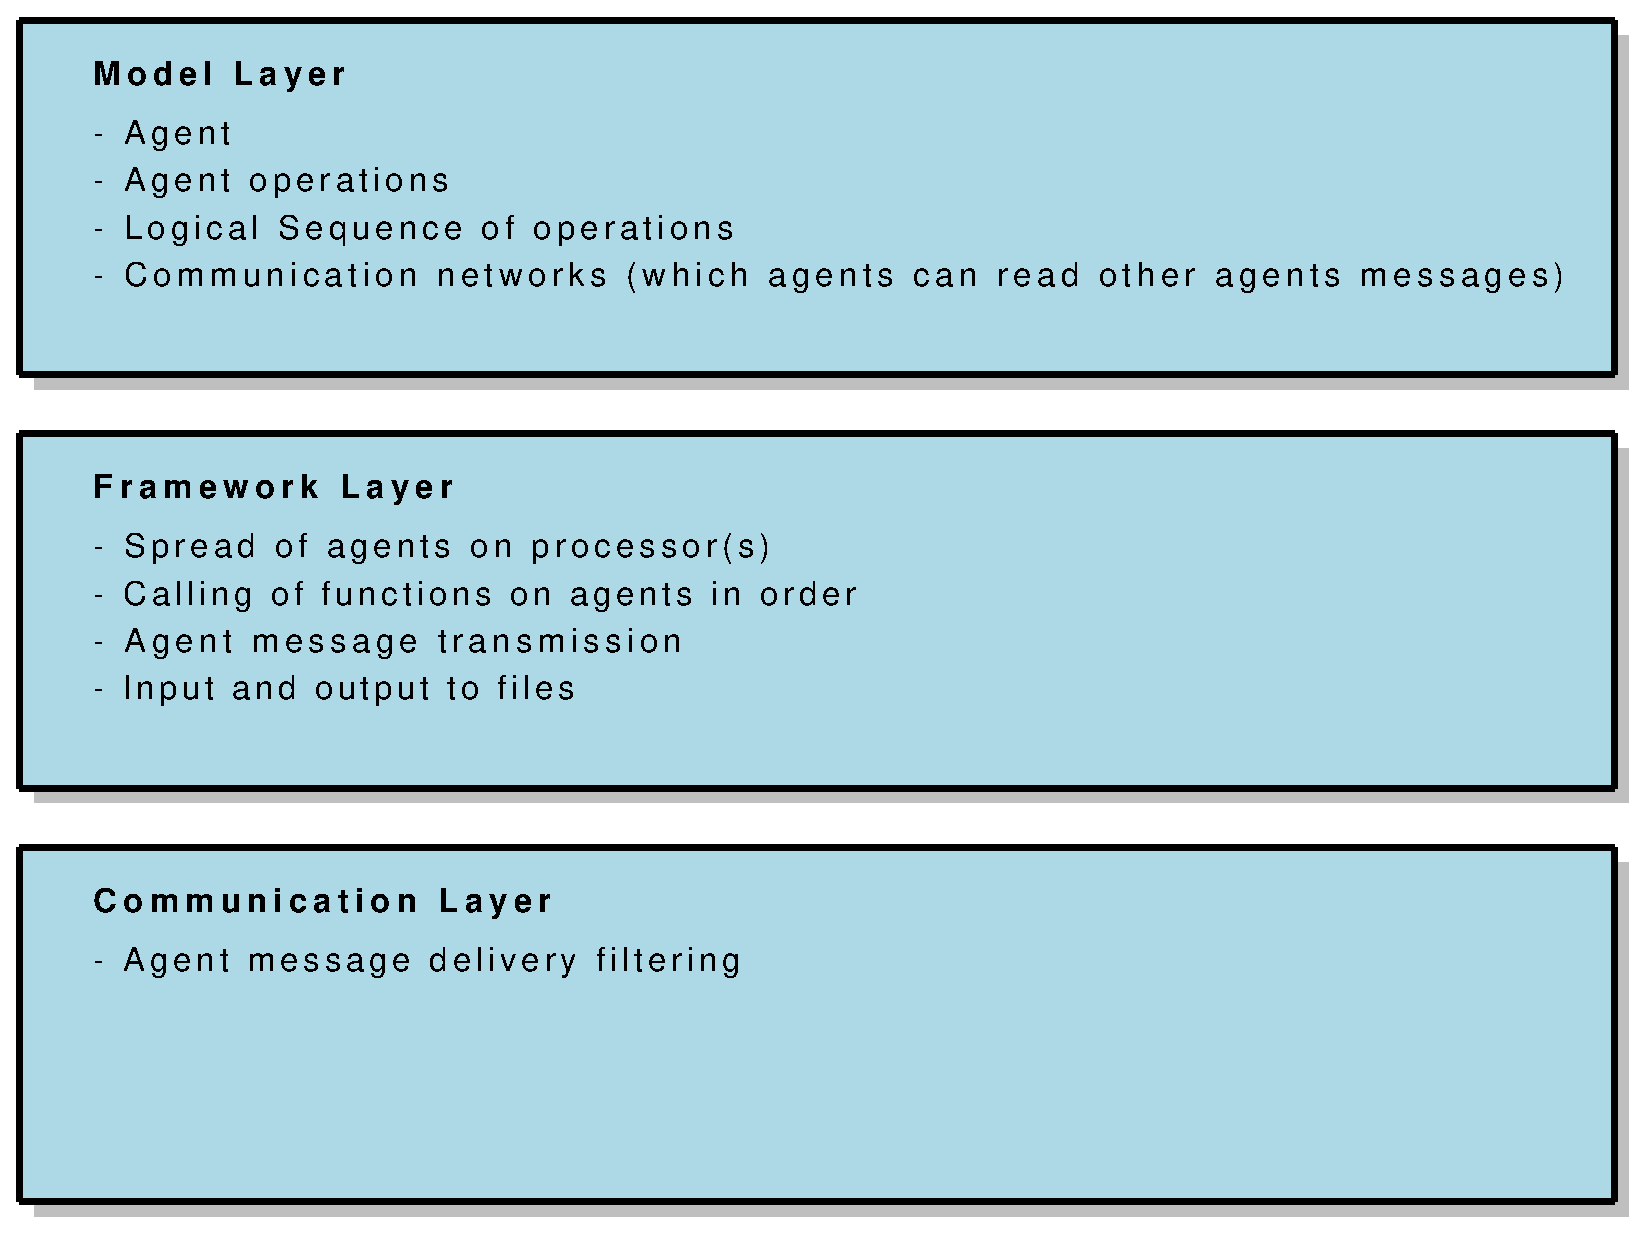
\includegraphics[width=\linewidth]{layers_1.eps}
\caption{Layers of abstraction for the framework.}
\label{fig:layers}
\end{center}
\end{figure}

\subsection{Handling Of Time}
\label{handlingoftime}

Computer simulations operate on two notions of time:

\begin{itemize}
\item The advancement of processing time
\item The advancement of simulation time
\end{itemize}

The processing time is the program progress and simulation time depends on program progress.
For agent-based simulations processing time is the processing of agents and the handling of communication.
Simulation time is advanced between periods of processing, for example when every agent is updated and all communication has reached its destination.

Deciding which agent to run and when to process/update it is a major issue.

For some theoretical results it can make a major difference in the outcome. The most dramatic example is the Game of Life where synchronous updates create patterns and structures capable of computation, but under an asynchronous scheme the model world quickly becomes lifeless. Another example comes from game theory where synchronous turns of players can evolve oscillation of states while asynchronous player turns quickly find a stable equilibrium \cite{HUBERMANGLANCE:1993}.

%Changing the order of the agents can produce different patterns.
Particularly for communicating agents is when communication completes, which is when messages are sent when are they available to be received.
This can involve two kinds of update strategies - synchronous, at the same time, and asynchronous, not at the same time.
These updates can be defined in the context of communication as follows:

\begin{itemize}
    \item Synchronous:
    \begin{itemize}
    \item Communication only completes after every agent is updated
    once.
        \item Order of agent updates does not matter.
    \end{itemize}
    \item Asynchronous:
    \begin{itemize}
    \item Communication completes after every agent is updated.
        \item Order of agent updates matters.
    \end{itemize}
\end{itemize}

\subsubsection{Communication}
Communication is very important when dealing with parallel
processing of simulations. It can act as a major bottleneck that can
slow down simulation times. Discussions with partners at STFC suggested that it
is the starting up and ending of communication between processors that is the major
factor and not the amount of data being sent \cite{HPCX:2003}. This suggests that the
least amount of communication synchronisation points, or completes, the better. It
also implies that it is better to send as much information as possible in a single communication than to send each piece of communication individually.

Deciding which computer platform to be used should not affect the results of a simulation.
Processing and communication time should affect simulation time and not in the other direction.
So the framework should be designed to be platform independent.
This becomes important when handling agent updating and communication.
In a simulation, agent communication should not be affected by the
number of processors used nor the physical
networks connecting them \footnote{The speed of the
cables or buses used for connection between processors responsible
for carrying agent communication}.
Summarising the points to be considered:

\paragraph{It should not matter that an agent is not on the same computing node.}
This requires all agent interaction is achieved via contactless communication via messages.
Contactless here refers to the inability to directly poll or access another agents memory values, as this is not possible if the agents are on a different computing nodes.

\paragraph{Any communication sent should be available for when it is needed to be read.}
This means operations that receive messages can only be run when messages have arrived.
The physical bandwidth of the communication hardware used to run a simulation will not affect the results.

\subsubsection{Updating Agents}
There are two ways an agent can be updated/processed.
Updating can be based on processing time information, called incremental based, or rely on incoming communication, called event based.
Though incremental based self updating can include incoming communication, and event based could include an incoming timed event.
%(note: Reference some papers from this group on event-based models and integrated formal methods)

Because agents only communicate via messages, they can be updated
at any time if any messages they need to read have
arrived. So the only thing affecting the updating of agents is the
communication dependencies, i.e. we can't update this agent until other agents have been updated.
By using the state machine
description to calculate the possible order of the functions, which
shall be called internal dependencies, and the communication input
and output between different functions, the communication
dependencies, a function dependence graph can be created.
A paper \cite{566188} from 2002 uses this dependence analysis technique to aid automated test case generation, which could also aid testing of models in the framework.
Figure \ref{fig:labour_fd} shows a dependency graph
for the labour market of all the actions that can happen in one day,
i.e. after a date event happens and waiting for the next one. From
the communication dependencies defined in the graph, one can add
stages where communication must complete before the corresponding
function requiring the input is processed. One can also assert that
an agent can be updated until it is waiting for incoming
communication and can only be updated again till after the
corresponding communication completes. The graph also shows what
agents need updated when, and depending what state they are in, the
function that is executed.

\begin{figure}
\begin{center}
\includegraphics*[width=6.0in]{labour_market_dependencies.eps}
\caption{Labour market function dependencies} \label{fig:labour_fd}
\end{center}
\end{figure}

\subsection{Communication Networks}
Parallel computation is easily handled when agents are communicating
via messages. The use of the idea of agent-agent and
agent-environment interactions is an abstraction above the
fundamentals. The only availability for agents communication are sending messages
and receiving messages.

\subsubsection{Agent-Environment Interaction}
The idea of an `environment' can be something that holds information
that could possibly change, which can be embodied as an agent
itself. Examples of environments in agent-based models can be:

\begin{itemize}
\item Land that grows crops (the ground cover environment).
\item Chemical signals (the chemical environment).
\item Newspaper business sections (the economic environment).
\end{itemize}

FLAME has been used for modelling biological systems, especially biological cells, 
where external solvers are needed to solve chemical diffusion and the physical movement of the cells.
It is functions in these `environment' agents that can be used to call external solvers, and pass back
information back to the cells.

\subsubsection{Agent-Agent Interaction}
Agent-agent interaction is when one agent sends a message and
another reads it. The agent reading messages can filter
messages depending on specified variables. Examples of which
include:
\begin{itemize}
\item Its `id' (direct).
\item Its `region' (local area interaction).
\end{itemize}

Agents do not need to hold a list of pointers to other agents to
represent their local neighbourhood. This can be achieved by the
following ways:
\begin{itemize}
\item Agents having the same region number.
\item Agents having a trade group number.
\item Agents having a location and filtering messages via a distance
metric.
\end{itemize}

Few instances, where the buyer has a preferred seller, such
information would be held within the agent memory. Networks in agent
based models are fully defined with agents, not a top down global
view.

%\subsection{Market Types}
%The various market types identified in economics are as follows:
%\begin{description}
%\item[Centralised (single intermediator)] All messages communicate through one agent. Even outgoing messages
%are thorough one agent.
%\item[Semi-centralised (multiple intermediators)] This depends on the choice of market
%interface used.
%\item[Decentralised (no intermediator)] Agents `pair' up to with each other to finish the work they are executing.
%\end{description}

%\subsection{Learning Mechanisms}

%Various agent-based models have introduced various learning
%mechanisms in agents. For this purpose various issues have to be
%considered.

%\subsection{Classification Of Learning Mechanisms}

\subsection{Simulation Output and Data Storage}

Data storage is an important issue. Currently data is being held in
XML format for ease of access but this presents problems with
increasingly large file sizes. Other
options to resolve this issue are being considered:

\begin{itemize}
\item Common Data Format (CDF) for the storage and manipulation of multi-dimensional data sets
\item Database which would also easier extraction of specific data
\item XML alternatives: YAML, JSON, SDL
\end{itemize}

Discussions and experiments with these and other file formats are currently being performed by Sheffield and STFC.
%[add recent work by Shawn and Susheel?]

\pagebreak

\section{Framework Implementation}

Initial work on implementation had already been undertaken by Simon Coakley as part of his Ph.D.
This involved creating a parser program that takes a model description as an input and produces a runnable simulation program, either in serial or parallel. Model descriptions are written in a file format called XMML which is a specific tag defined XML file. The XML format provides a structure for data that computers and humans can understand. A model description file allows metadata about a model to be used to direct source code creation (via a parser program), especially for parallel code that modellers do not need to encounter. It can also be used to direct testing efforts and produce diagrams of a model that aid in its understanding.

\subsection{Xparser}
The Xparser is the name of the program that reads XMML model files
and produces simulation program code, see Figure \ref{fig:xparser}.
Additional features that have been added since the project started include:

\begin{itemize}
\item Function dependencies -- agent functions can now be ordered in such a way that the simulation program can execute them at the best possible moment (which is calculated), and allows for future use of threading techniques.
\item Template engine -- the logic behind the generated simulation code has been transfered to template files so that collaboration between partners is easier.
\item Dynamic arrays for agent memory -- the ability to have dynamic sized arrays in agent memory has been added (although movement of agents on a parallel machine used for load balancing has yet to be implemented).
\end{itemize}

The Xparser also has an XML reader to read the XMML model descriptions, and also generates graphs of the function dependencies for analysis.

\begin{figure}[!htb]
\begin{center}
\includegraphics*[scale=0.5]{xparser.eps}
\caption{Xparser usage}
\label{fig:xparser}
\end{center}
\end{figure}

The Xparser is completely written in C with the use of standard libraries only. This was so that the program could be deployed on any platform (with a C compiler) simply and easily. Because most of the logic is held in the simulation template files it is viable to create a program in any language or use additional libraries that would do the same job as the Xparser.

\subsubsection{Process Sequence}

Agent functionality is defined by its functions. Functions change
the agent state and drive a simulation forward. The sequence that
these functions are run is determined by their dependency on each
other, defined in the model XMML. Dependencies are either
communication, dependent on messages, or internal, dependent on
agent internal memory.

It is possible to construct a dependency graph (a directed acyclic
graph) to show the sequence of events that happen in a simulation.
Whenever a communication dependency occurs, in parallel, this
requires a synchronisation block between the nodes so that messages
arrive in time to meet the dependency. These synchronisation blocks
are a major time bottle neck and so the fewer there are the more
efficient the simulation. By traversing a dependency graph it is
possible to calculate the most efficient time to run functions and
where best to place synchronisation blocks.

Creating the function dependency graph currently uses a simple
algorithm. It finds functions with no dependencies on it, assigns
them a layer, removes them from the graph, and reruns the algorithm.

Figure \ref{fig:d1example} shows eight functions with dependencies. All are
communication (denoted with a `C') except the dependency of
Function 2 on Function 5 which is internal (denoted with an
`I'). Because internal dependencies do not need a
communication synchronisation block we can organise the
synchronisation blocks in such a way that we need the least amount of
them. An example of this strategy is the organisation of the functions from Figure \ref{fig:d1example} into layers separated by synchronisation blocks in Figure \ref{fig:dsyncexample}.

\begin{figure}
\begin{center}
\includegraphics*[scale=0.5]{example_dgraph_1.eps}
\caption{Communication dependencies between functions}
\label{fig:d1example}
\end{center}
\end{figure}

\begin{figure}
\begin{center}
\includegraphics*[scale=0.5]{example_dgraph_1_sync.eps}
\caption{Syncing communication dependencies as synchronisation layers}
\label{fig:dsyncexample}
\end{center}
\end{figure}

\subsection{Framework Communication}

The usual attribute that separates agent-based models from other modelling techniques (like differential equations) is the use of space. Agents have a location attribute that places them in space in relation to other agents. To create new results from this added dimension of space, communication is usually restricted to a distance metric, so that information is kept localised. This knowledge can be used to direct efficient communication in a model implementation.

%Message communication efficiently in agent-based models is known that agents usually only read a subset of all the messages sent in a simulation.
%This is mainly due to localised communication.

Currently to efficiently handle messages with respect to localised communication:
The current implementation of the framework is based around the idea of space as a Cartesian scale in 1, 2 or 3 dimensions, with:

\begin{itemize}
\item All agents defined with a Cartesian location
\item All messages are defined with originating Cartesian location and range
\item Agent space is partitioned along Cartesian lines
\end{itemize}

In this way when a message is sent by an agent, the message can be defined as originating from the agent location and can only be read by agents with location that is defined within the message range. To aid efficiency messages are only sent to partitions in agent space that include agents within the message range. After discussions with members of the STFC unit about parallel communication in HPCs the filtering of messages that are to be sent to different nodes is not required. Firstly that filtering of messages is done twice, when messages are sent between nodes, and when agents try and read incoming messages. Secondly that the filtering of messages before they are sent between nodes is unnecessary. This is because the time cost of sending messages between nodes is more weighted on the opening and closing of communication and less on the actual amount of data that is sent \cite{HPCX:2003}, this iterates the importance of keeping communication synchronisation blocks to a minimum. Therefore it is more efficient to send all out going communication to all nodes. This then shifts all efficiency efforts onto the filtering of messages for agents to read. This strategy is mentioned in Section \ref{sec:unimodframework}.

Also in efforts to make the framework more generic the idea of space should not be restricted by a Cartesian scale, or in fact any distance scale. This is because agent space might be defined as groupings, for example NUTS-2 regions.

%\subsubsection{Parallelisation}



%By stipulating communication via messages, and function dependencies, the framework is inherently parallelable. This is because the agents have been defined as singular processes that only communicate with messages. This allows agents to be placed on different nodes with messages sent between nodes. Function dependencies are used to make sure messages have arrived before a function is run that reads them.

\subsection{X-Machine Agent Markup Modelling Language (XMML)}

A description language for agent-based simulations, XMML has been
presented here. XMML is orientated towards representing agent-based
models as formalised abstract state machines, particularly
communicating X-machines. The motivation was to provide a formalised
framework to enhance creating and testing of agent-based models and
also provide innate parallel processing capabilities.

\subsubsection{Features of XMML}

There are a number of factors which make XMML unique to achieve its
research purposes. A few have been listed below:
\begin{itemize}
\item XMML is not restricted by research area.
\item It is not restricted by any grid or location based structure.
\item Communication is not restricted between agents, but mechanisms are available to efficiently filter incoming messages.
\item Agents are updated at the most efficient time and in parallel (if available)
%\item Currently simulation time is incremental based, advanced in regular time steps, such that agents have an order that they run rules (functions).
%Future work will look at implementations that are event based, simulation time is advanced depending on the next timed event.
%\item XML examples are written in a typewriter-style font.
\end{itemize}

XMML is meant to aid agent-based modellers in developing more
formalised models that are easier to create, test, share, and be
parallel processable without additional work. The definition of the
model description language here does not specify how to parse the
model description into a simulation program but defines what is
required and how the simulation is advanced.

\subsubsection{Data}

Variables represent the data that is possessed by the agent in their
memory and the messages they send or receive. While executing a
simulation program the details of this data needs to be known in advance. The advantage of this approach are that data structures and algorithms that handle data, especially in parallel, can be automatically generated:

\begin{itemize}
\item Creating data structures for agents and messages
\item Creating functions that handle input and output to files
\item Creating functions that access agent memory
\item Creating functions that interact with messages
\item Creating parallel algorithms that handle data between nodes
\end{itemize}

Variables contain a data type and a name. Data types are used to assign storage for the variable and define the type of data that will be held in that location. Variable names are used to reference and alter the data if needed. The following XML represents a variable of type \emph{float} and named \emph{temperature}.

\begin{mylisting}
\begin{verbatim}
<var>
  <type>float</type>
  <name>temperature</name>
</var>
\end{verbatim}
\end{mylisting}

\subsubsection{C Language}
The current XMML to simulation code parser is written in the C programming language, therefore allowing C data types to be used. Examples of these have been given in Table \ref{tab:cdata}.

\begin{table}[hbtp]
\centering
\begin{tabular}{|l|l|l|l|}
\hline
Type & Description & Usual Byte Size & Example Usage\\
\hline \hline
int & Integer number & 2 bytes & int count;\\
& & & count = 5;\\
\hline
float & A single-precision floating & 4 bytes & float temp;\\
&  point value & & temp = 6.2;\\
\hline
double & A double-precision floating & 8 bytes & double sun\_temp;\\
&  point value & & sun\_temp =\\
&&&13600000.0;\\
\hline
char & Character & 1 byte & char letter;\\
& & & letter= `a';\\
\hline
\end{tabular}
\caption{C fundamental data types.} \label{tab:cdata}
\end{table}

\subsubsection{Data Structures}
To facilitate more structured data representation, new custom data
types can also be created. These custom data types can allow C data
types as well, and they can be referred to by their own user defined
names. Table \ref{tab:empdata} gives an example of a custom data
type called \emph{employee} which holds an `id' of type \emph{int}
and a `wage' of type \emph{float}.

\begin{table}
\centering % used for centering table
\begin{tabular}{|l|}
\hline
$<$datatype$>$\\
$<$name$>$employee$<$/name$>$ \\
$<$desc$>$Used to hold employee information$<$/desc$>$\\
$<$var$><$type$>$int$<$/type$><$name$>$id$<$/name$><$/var$>$\\
$<$var$><$type$>$float$<$/type$><$name$>$wage$<$/name$><$/var$>$\\ $<$/datatype$>$\\
\hline
\end{tabular}
\caption{Example of the employee data type.} \label{tab:empdata}
\end{table}

The $<$desc$>$ $<$/desc$>$ tags can be used to allows users to
describe the data type which can later be extracted to be used for
description in the documentation. These custom data types can now be
used in the same way as the C data types.

\subsubsection{Array}
Variables can also be defined as a list which can also be
represented as an array. The array can either be static, with
predefined size, or dynamic, allowing its size to change. To define
a static array, use the C syntax which is to place square brackets
after the variable name that contains the array size. So for a list
of six variables of type float called wage, the definition would be
(Table \ref{tab:array1}):

\begin{table}[!htp]
\centering % used for centering table
\begin{tabular}{|l|}
\hline
$<$var$><$type$>$float$<$/type$><$name$>$wage[6]$<$/name$><$/var$>$\\
\hline
\end{tabular}
\caption{Defining an array of predefined size.} \label{tab:array1}
\end{table}


Dynamic arrays have their own special data type provided by the
XMML. For any data type name just add `\_array' at the end.
Therefore to change the static array above to a dynamic array, take
away the square brackets and size and add `\_array' to the data type
name (Table \ref{tab:array2}):

\begin{table}[!htp]
\centering % used for centering table
\begin{tabular}{|l|}
\hline $<$var$><$type$>$float\_array$<$/type$><$name$>$wage$<$/name$><$/var$>$\\
 \hline
\end{tabular}
\caption{Defining a dynamic array.} \label{tab:array2}
\end{table}


\subsubsection{XMML Components}
XMML components are the representation of how models are described
in its specification. The description comprises of the agents
involved, the agent characteristics and the messages being used to
communicate among the agents.

\subsubsection{Agents}

Every agent is a X-machine. This depicts that the agent would thus
contain a set of memory variables which it can update during its
functions. The agent would also have a set of functions it can
perform. The actual function definition is not part of XMML
component and is defined separately in a C file. Table
\ref{tab:firmdata} gives an example of a firm agent.


\begin{table}
\centering % used for centering table
\begin{tabular}{|l|}
\hline $<!--*******$ X-machine Agent - Firm $**********-->$\\
$<$xmachine$>$\\
$<$name$>$Firm$<$/name$>$ \\
$<!---------$Variables$------------>$\\
$<!--$ All variables used by Firm are declared\\
here to allocate them in memory $-->$\\
$<$memory$>$ \\
$<$var$><$type$>$int$<$/type$><$name$>$id$<$/name$><$/var$>$\\
$<$var$><$type$>$double$<$/type$><$name$>$value$<$/name$><$/var$>$\\
$<$/memory$>$\\ $<!-----------$ Defining functions
$------->$\\
$<$functions$>$\\
$<$function$><$name$>$Firm\_1$<$/name$><$/function$>$\\
$<$function$><$name$>$Firm\_3$<$/name$><$/function$>$\\
$<$/functions$>$ \\$<$/xmachine$>$\\
 \hline
\end{tabular}
\caption{Example of a Firm Agent.} \label{tab:firmdata}
\end{table}

\subsubsection{Messages}
Messages are used to communicate between the agents. All messages
are enclosed in the $<$messages$>$ $<$/messages$>$ tag and every
message structure is defined seperately. An example has been shown
in Table \ref{tab:msg}.

\begin{table}
\centering % used for centering table
\begin{tabular}{|l|}
\hline $<$messages$>$\\ $<!---$Message for stock of the firm$----->$ \\
$<$message$>$ \\$<$name$>$firm\_stock$<$/name$>$\\
$<$note$>$This message lets the people know how much stock\\
the firm they are buying from has left.$<$/note$>$\\
$<$var$><$type$>$int$<$/type$><$name$>$firm\_id$<$/name$><$/var$>$\\
$<$var$><$type$>$int$<$/type$><$name$>$stock$<$/name$><$/var$>$\\
$<$/message$>$\\ $<$/messages$>$\\
 \hline
\end{tabular}
\caption{Example of describing messages.} \label{tab:msg}
\end{table}

\pagebreak
\clearpage

\section{Model Creation}

\subsection{Data structures}
From the definitions in model XMML data structures can be created
for agent memory and message memory.

Agent and message memory is made up of variables of certain data
types. These can be:
\begin{itemize}
\item C fundamental data types - int, float, double, char (Table
\ref{tab:cdata}).
\item Abstract data types made up of more than one C data type.
\item Static arrays of C data types and abstract data types.
    \item Dynamic arrays of C data types and abstract data types.
\end{itemize}
Dynamic arrays are a built-in feature of the framework (for sending
messages in parallel the size of the array is needed). For any data
type just add `\_array' to the end, and access it via the following
functions:
\begin{itemize}
 \item datatype\_array * my\_array = init\_datatype\_array();
    \subitem For initialising the array.

\item add\_datatype(my\_array, value);
\subitem For adding an element to the array.

\item remove\_datatype(my\_array, index);
\subitem For removing element at
the specified index.
\item my\_array-$>$size; \subitem for returning the length
of the array. \item free\_datatype\_array(my\_array); \subitem For
freeing the array.
\end{itemize}

\subsection{Definition of XMML tags}

The model description is given in the XML file using XMML tags which
have been described previously. These tags are used by the xparser
to recognise the agent memory, the sort of variables being used and
the functions they can perform.
\subsection{Handling Variables in Agent
Memory}

The xparser offers a few functions which can be used to access the
variables in the agent memory. \begin{itemize}
\item set\_variablename(\emph{value})
\end{itemize}

The set function can be called with in the agent function to change
the value of the variable in the memory. The following brackets
contain the value to be replaced with. \begin{itemize} \item
x=get\_variablename()
\end{itemize}
The get function can be called within the agent function and gets
the value of the variable wanted and saves it to the local $x$
value.
\subsection{Handling Messages}
\begin{itemize}
\item add\_messagename\_message(\emph{var1, var2,}...)
\end{itemize}
To add the message onto the message board. \emph{Var1, var2}
symbolize the value of the variables that the message carries.
\begin{itemize}
\item messagename\_message=get\_first\_messagename\_message()
\end{itemize}
The local variable gets the first message to traverse through the
message.
\begin{itemize}
\item messagename\_message-$>$\emph{var1}
\end{itemize}
The above command allows you to get the value of \emph{var1} from
the message.
\begin{itemize}
\item messagename\_message =
get\_next\_messagename\_message(messagename\_message);
\end{itemize}
The above command allows the loop to move onto the next message on
the board to read through. This would be used with a while loop
until it returns a \emph{null}.

\subsection{Handling Dynamic Arrays}

The framework allows dynamic arrays to be used within the memory of
the agent. This is useful when the agent needs to maintain a list of
a continually growing nature of variables.
\begin{itemize}
\item int\_array * Agents = init\_int\_array()
\end{itemize}
The above command initializes the dynamic array.
\begin{itemize}
\item xmachine\_memory\_agentname * xmemory =
current\_xmachine-$>$xmachine\_agentname;
\end{itemize}
To access the memory the xmemory pointer needs to be used with the
current xmachine to point to the xmachine being accessed. The
pointer would be of the type of the agent being accessed.
\begin{itemize}
\item reset\_int\_array(xmemory-$>$dynamicvariablename);
\end{itemize}
When accessing the dynamic variable array we can use the reset to
reset the array.
\begin{itemize}
\item add\_int(xmemory-$>$dynamicvariablename, messagename\_message-$>$var1);
\end{itemize}
To add to the dynamic array list use the above command with the name
of the array given first and the value after the comma.
\begin{itemize}
\item xmemory-$>$dynamicvariablename-$>$array[value]
\end{itemize}
Values in the dynamic array can be accessed similar to the way
elements in an array would be accessed.
\begin{itemize}
\item xmemory-$>$dynamicvariablename-$>$size
\end{itemize}
The size can be used to return the value of the size of the array.
This would be changing continually as it is not fixed.
\begin{itemize}
\item free\_int\_array(agents);
\end{itemize}
To free the list of the agents used.

\subsection{Outputs Produced by the Xparser}

The Xparser produces simulation source code files, a compilation script, and a documentation options file. 
Also produced are two graphs that show function dependencies (see Figures \ref{fig:dg1}, \ref{fig:dg2} for examples) and function order with communication layers (see Figure \ref{fig:casff} for an example).

%Order of agent functions (creating a dependency graph from the function dependencies). Figures \ref{fig:dg1}, \ref{fig:dg2} are examples of the outputs produced.

%The svg files, produced after compilation with the xparser, allow a clear understanding on how the functions will be ordered during execution. Figure \ref{fig:casff} depicts the output of the svg files. The red points depict a synchronisation point, at which point the functions prior to it would have finished executing and sent out messages which the later functions can then read and proceed.

%This figure also depicts how the functions will be distributed in a parallel manner. more than one function in the layer can be run on more nodes and all information could be brought together at the synchronisation point.

\pagebreak

\section{Understanding Economic Models: The C@S Model}

The first effort to create an economic model centred around the C@S
project with papers in progress provided by the Ancona unit \cite{CATALANO:2006}. The model describes
a sequential economy populated with large numbers of firms and
workers/consumers who partake on markets for homogeneous
non-storable consumption goods and labour services.

Newly introduced into the model was the idea of locality, at the
heart of parallelising efforts. Where agents were given a location
on a two dimensional continuous plane. The distance between agents
in this Cartesian space affected if they could communicate with each
other.

%[SIMON TO DO] Introduce locality

\subsection{Version 1: Without the Mall Agent}

From the paper describing the C@S model, two agents Firm and Person were implemented. Table \ref{tabcas} shows the relation between the event sequence described in the paper and the order of the agent functions.
The importance of this version is that only one agent function is used
when firms hire workers and persons buy goods. This is achievable
only because these functions are run sequentially, and are therefore
not parallelable. They depend on messages sent by the running of the
function on other agents, and is therefore a self-dependency. The means the
function needs to be run one after the other with messages sent
available immediately to the consequent function run on other
agents. The self-dependency is shown in the functions 'Firm\_3' and 'Person\_5' in the function
dependency diagram in Figure \ref{fig:dg1}.

\begin{table}[hbtp]
\centering
\begin{tabular}{|c|c|l|l|}
\hline
Function&Event&Firm Agent&Person Agent\\
(model)&(paper)&&\\
\hline \hline
1&1,2,3&Checks financial viability&Does nothing\\
&&Calculates production&\\
&&Calculates labour required&\\
&&Send price inflation message&\\
\hline
2&4&Does nothing&Calculate total price inflation\\
&&&(from price inflation messages)\\
&&&Calculate new wage\\
&&&Send job application messages\\
\hline
3&5&Hire workers&Does nothing\\
&&(from job application messages&\\
&&and send hired messages)&\\
\hline
&6&&\\
\hline
4&7a&Calculate wage bill&Check hired messages\\
&&Calculate goods price&(update status if hired)\\
&&(send price message)&\\
&&Calculate produced goods&\\
&&(send stock amount message)&\\
\hline
5&7b&Does nothing&Spend income on goods\\
&&&(using firms price and stock\\
&&&messages, send updated stock\\
&&&messages if buying)\\
\hline
6&8&Calculate stock sold&Add wage to income\\
&&(from stock messages)&(for next iteration)\\
&&Calculate revenue&\\
&&Calculate profits&\\
\hline
\end{tabular}
\caption{Sequence of events in the C@S model} \label{tabcas}
\end{table}

\begin{figure}
\begin{center}
\includegraphics*[scale=1.5]{cats_dgraph_v1.eps}
\caption{Function dependency graph of C@S model version 1}
\label{fig:dg1}
\end{center}
\end{figure}

\subsection{Version 2: With the Mall Agent}

The second version included a new agent type (defined by the XMML in Appendix \ref{cats_model_xmml}). The mall agent was
introduced to parallelise the labour and goods markets and also to make
the markets fairer as the cheapest workers and goods would be evenly
distributed rather than first come take everything approach of
version one. It also added locality of agents and the feature that firms and persons had to
choose which mall to go to for the labour market and the goods
market. The function dependency graph of this model is shown in Figure \ref{fig:dg2}.
Figure \ref{fig:casff} shows the communication
synchronisation points between the different functions of the agents. The diagonal lines represent the points at
which all functions prior to it would need to be finished for the simulation to proceed.

\begin{figure}
\begin{center}
\includegraphics*[scale=1.5]{cats_dgraph_v2.eps}
\caption{Function dependency graph of C@S model version 2}
\label{fig:dg2}
\end{center}
\end{figure}

\begin{figure}
\begin{center}
\includegraphics*[scale=1.0]{cats_v2_com_layers.eps}
\caption{Communication synchronisation layers of C@S model version 2} \label{fig:casff}
\end{center}
\end{figure}

\subsubsection{Graphs}

The graph in Figure \ref{fig:g1} represents the pattern of behaviour between the
goods sold, price and the production. when the price increase the
goods sold reduces which causes a reduction in the production.
Simultaneously if the price is low, more goods are sold causing more
production to take place.

\begin{figure}
\begin{center}
\includegraphics*[width = \linewidth]{g1.eps}
\caption{Graph showing the relation of price, stock sold, and
production} \label{fig:g1}
\end{center}
\end{figure}

Graph \ref{fig:g2} shows the relation of wages, price, production
and goods sold. The price of the goods denotes a price inflation
when the price has increased in the previous iteration. With an
increase in price the wage of the workers increase as they demand
higher wages. The goods sold and the production seem to have a
mirror relation between them. When goods sold increase production
increases and vice versa. The interesting facet about this relation
is that the two seem to reach an equilibrium even if the are greater
fluctuations in the wage and the price.

\begin{figure}
\begin{center}
\includegraphics*[width = \linewidth]{g2.eps}
\caption{Graph showing the relation between average wage,
price, production, and the stock sold} \label{fig:g2}
\end{center}
\end{figure}

\pagebreak

\section{Building Eurace by Markets}

\subsection{The Labour Market Model}

The labour market was initially described in a document by the
Universitaet Bielefeld unit. This describes a matching algorithm
between job seekers and vacancies in a six step approach. Initially
each step was assigned per day in a simulation.

\begin{table}[hbtp]
\centering
\begin{tabular}{|c|p{2.0in}|p{2.0in}|}
\hline
Step & Firm & Household\\
\hline \hline
1 & Send Vacancies & \\
\hline
2 & & Read Vacancies\\
\hline
3 & Read applications, rank, and send job offers &\\
\hline
4 & & Read job offers,rank and send job acceptance\\
\hline
5& Read job acceptances & \\
\hline
6 &Update wage offer & Update reservation wage\\
\hline
\end{tabular}
\caption{Six step labour market algorithm.} \label{tab:6step}
\end{table}

At the Bielefeld working meeting the following were discussed:
\begin{itemize}
\item Communication between agents happen between agent functions:
\begin{itemize}
          \item One agent function sends a messages, and another agent function reads the
          message.
          \end{itemize}
\item When one function depends on a message sent from another
function this is called a communication function dependency.
\item When one function depends on the outcome of another functions within in the same agent this is called an internal function dependency.
    \item Function dependencies are not allowed to happen across time steps
    (days).
         \begin{itemize}
         \item Because each day is taken to be a separate simulation run (this removes many
         problems).
\end{itemize}
\end{itemize}

\begin{figure}
\begin{center}
\includegraphics*[width = \linewidth]{labour_1_eps.eps}
\caption{Blackboard diagrams describing discussions on the labour market model} \label{fig:blackboard_lmm}
\end{center}
\end{figure}

As a group task the function dependencies of agent functions where
discussed and written on a black board. This started to produce
pairings of functions where communication needs to happen. These
were written as arrows with a capital `C' to denote a communication
dependency. The six step algorithm then became four function
communication dependency pairs, see Figure \ref{fig:bb}.

\begin{figure}
\begin{center}
\includegraphics*[width = \linewidth]{labour_maket_day_by_day.eps}
\caption{Function dependency of the labour market day by day} \label{fig:bb}
\end{center}
\end{figure}

After some discussions which included time scales, firm production
frequency and overlap, it was decided that the whole labour market
model would act completely every day. This allowed one function
dependency graph to describe the total labour market algorithm. This
was written up in XMML as a model description, see Appendix \ref{labour_market_model_xmml}.

\begin{figure}
\begin{center}
\includegraphics*[width=2.5in]{labour_market_bielefeld_dgraph.eps}%{labourdgraph.eps}
\caption{Function dependency graph of the labour market} \label{fig:labdgraph}
\end{center}
\end{figure}

%Where each agent functionality was given a separate function `box'. In fact if there is only an internal dependency between agent functions, both functions can be merged, as has been done for the first implemented version.
\subsubsection{Agents}

The agent types used, their behaviour, and their forecast number in the labour market are:
\begin{itemize}
\item Household - looking for a job - 1000
    \item Firm - looking to fill vacancies - 100
    \item Market Research - sends market data to firms - 1
\item Eurostat - sends high wage information to firms - 1
\end{itemize}
Which corresponds to one region or NUTS-2 regions.

\subsubsection{Function Layout}

All internal function dependencies have been removed where they are
the only dependency and the functions merged. This creates a more
compact and easier to read model. It also saves memory space as
creating lists (of vacancies, application, and job offers), ranking,
and deleting them can all be done locally in the same function
without saving the list to agent memory.
\begin{figure}
\begin{center}
\includegraphics*[width=\linewidth]{labour_market_0.1_dgraph.eps}
\caption{Updated function dependency graph of the labour market} \label{fig:xalm}
\end{center}
\end{figure}

\subsubsection{Implementation}

The labour market revolves around the monthly cycle of firms
calculating their monthly production. On the day of month they
calculate this they ask the eurostat agent and market research agent
for additional information then calculate the number of employees
they need. If they have too many employees they send redundancy
messages out, and if they have too few they send out vacancy
messages.

\subsubsection{Results and Conclusions}

The labour market model provides a test bed to research:
\begin{itemize}
\item Ways to design models
\begin{itemize}
          \item Function dependencies
          \end{itemize}
\item Ways to implement models
\begin{itemize}
          \item Cluster internal functions
          \end{itemize}
    \item Ways to run models efficiently
\end{itemize}
Running models efficiently includes calculating when best to run
functions and where to place communication synchronisation points
between functions. Figure \ref{fig:xalmsync} lists the functions on rows with
communication points as diagonal lines. This is the order the functions
will be run in with communication handled at the red lines. The main
efficiency to be gained is to have as few amount of communication
points as possible, as this is the main bottle neck in parallel (the
starting up of communication between nodes).


\begin{figure}
\begin{center}
\includegraphics*[scale=0.7]{labour_market_com_layers.eps}
\caption{The communication sycnronisation layers of the labour market model} \label{fig:xalmsync}
\end{center}
\end{figure}

As part of handling messages efficiently the message board will
automatically organise messages in relation to the filters agents
use to read messages, for example with a distance metric.

\subsection{The Asset Market Model}

Also discussed at the Bielefeld work meeting, the asset market is
still under construction. Figures \ref{fig:hh1} and \ref{fig:p1} depict the block diagrams of the
market and how it functions\footnote{These figures are a result of the discussion at the Bielefeld work meeting and converted into figurative form by Sander van der Hoog from the GREQAM unit.}.

\subsubsection{Agent Population}
\begin{description}
\item[Household Agent.] Invests in assets.
\item[Firm Agent.] Issues assets (stocks and bonds).
\item[Financial Advisor Agent.] Gives advice to households on the past performance of a set of asset allocation rules. It holds a database of such rules in its internal memory.
\item[Asset Management Company.] A firm that manages Exchange Traded Funds (ETFs) and/or hedge funds. Like other firms, the Financial Advisor distributes its profits to its shareholders. There can be multiple Financial Advisors.
\item[Clearinghouse Agent.] Reads limit\_order\_messages. Computes transaction prices.
\item[LimitOrderBook Agent.] Reads limit\_order\_messages. Computes transaction prices.
\end{description}

\subsubsection{Internal Dependencies}
A few internal dependencies in the household and the firm agent have
been identified. These have been depicted in the dotty diagram in
Figure \ref{fig:hh}.

\subsubsection{Implementation}
The asset market works on a monthly basis as depicted in Figure
\ref{fig:hh1}. The diagram shows that it starts on the first day of
the month and continues normal procedure for the rest of the month.
The first column, however, depicts how the asset market connects to
the markets outside its own realm, like the `Consumption Goods
Market (CGM)' and external agents as the banks and the firms. A few
implementation issues were encountered as listed below:
\begin{description}
\item[Problem of \emph{Days}.] Figure \ref{fig:hh1} shows how some
of the functions of the asset market have to be run on one day on
the month with the rest of the functions running as normal. \subitem
This gives rise to the discussion on how long is one simulation
supposed to be depicted for. To make it default, USFD has proposed
to make the length of one simulation to depict one day. \subitem
There is another issue on how the date of the day will be checked as
some of the functions are dependent on which day of the month it is.
Discussions with the STFC unit have led to a few conclusions of
either including a date check in every function description or the presence of a date agent allowing some functions to be
executed. Further tests will be done to find the most efficient
manner of doing this.
\item[Internal and message dependencies.] Figure \ref{fig:p1} depicts the function
dependencies to be of two types - {internal} or {message}. As
previously discussed on communication dependencies, internal
represents dependency on functions within the agent. Thus some of
these functions can be combined into one.
Combining functions allows possibly more efficient use of memory and a more readable function dependency graphs, but removes the possibility of parallel execution (by future use of threads) and the ease of testing smaller functions.
The external {message} dependency
, is when the agent depends on another agent for data.
Therefore these would be the synchronisation point at which prior to
it all agents would have finished working and wait to move into the
next block. The importance of reducing the layers to {message}
dependencies reduces the synchronisation points to be encountered.
this reduces computational overhead in the model.

\end{description}

\subsubsection{Current Work}
The model has already been designed and implemented in MATLAB by the
Genoa unit in collaboration with the GREQAM unit and is going to be converted into C language for
implementation using the framework.

\clearpage

\begin{landscape}

\begin{figure}
\begin{center}
\includegraphics*[width = \linewidth]{hh.eps}
\caption{Dotty diagram of household and firms.} \label{fig:hh}
\end{center}
\end{figure}

\begin{figure}
\begin{center}
\includegraphics*[width = \linewidth]{hh1.eps}
\caption{Function dependency graph for the Financial Management Role
of the Household.} \label{fig:hh1}
\end{center}
\end{figure}

\begin{figure}
\begin{center}
%\includegraphics*[width = \linewidth]{portfolio1.eps}
\includegraphics*[width = \linewidth]{Portfolio_selection_algorithm_layers.eps}
\caption{Function dependency graph for the Portfolio Selection
Algorithm of the Household.} \label{fig:p1}
\end{center}
\end{figure}

%\begin{figure}
%\begin{center}
%\includegraphics*[width = \linewidth]{portfolio2.eps}
%\caption{Function dependency graph for the Portfolio Selection
%Algorithm of the Household, showing the three communication layers.}
%\label{fig:p2}
%\end{center}
%\end{figure}

\end{landscape}

\pagebreak

\appendix
%\include{xml_schema}
\section{XMML Schema}
\label{cha_xmlschema}
\small{{\tt \verbatiminput{xmml.xsd}}}

\pagebreak

\section{C@TS Model}
\label{cats_model_xmml}
\small{{\tt \verbatiminput{C@S.xml}}}

\pagebreak

\section{Labour Market Model}
\label{labour_market_model_xmml}
\small{{\tt \verbatiminput{labour_market.xml}}}

\pagebreak

%\bibliographystyle{socreport}
%\bibliographystyle{elsart-harv}
\bibliographystyle{plain}
%\bibliography{example}
\bibliography{EURACE_refs}
\addcontentsline{toc}{section}{References}

\pagebreak

\section*{Glossary}
\label{glossary}
\addcontentsline{toc}{section}{Glossary}

\begin{description}
\item[Eurostat]: The statistical arm of the European Commission.
\item[HPC]: High Performance Computer -- parallel supercomputer or computer cluster.
\item[Node]: Any single computer connected to a network. Supercomputer clusters are many up of many nodes.
\item[NUTS-2]: Nomenclature of Territorial Units
for Statistics -- Used by Eurostat for E.C. regional statistics, level 2 being the region level.
\item[UML]: Unified Modelling Language -- a standard notation and modelling technique for modelling software systems.
\item[XML]: Extensible Markup Language -- a simple and very flexible text format designed for information exchange that encodes data with meaningful structure and semantics.
\end{description}


\end{document}
